\begin{surferPage}{奇穆托夫8次曲面}
乍一看上去,奇穆托夫8次曲面$\text{Chm}_{d}, \ d=8,$具有明显的对称性。这也能从它的定义方程看出来:\[\text{Chm}_{d}\colon T_d(x) + T_d(y) + T_d(z) + 1 = 0,\]其中$T_d$是所谓的车比雪夫多项式(左图)。曲线$T_8(x)+T_8(y)=0$是右图。
     \begin{center}
      \begin{tabular}{c@{\quad}c}
        \begin{tabular}{c}
          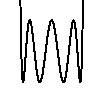
\includegraphics[height=1.75cm]{./../../common/images/Tcheb_008.pdf}
        \end{tabular}
        &
        \begin{tabular}{c}
          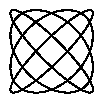
\includegraphics[height=1.75cm]{./../../common/images/Tcheb_2d_008.pdf}
        \end{tabular}
      \end{tabular}
    \end{center}
    \vspace{-0.3cm}
从这些图到交互式图中的曲面形状也就几步之遥。

这些方程由奇穆托夫在上世纪80年代给出。对大多数$d$, 由他们构造的$\mu(d)$成为了当时的世界纪录。
上世纪90年代,奇穆托夫更新了他自己的纪录。2005年,布莱斯克,莱布斯与范斯滕森利用这个构造产生了只有实奇异点的实曲面。
\end{surferPage} 
